% Source: Wald GR, physical PDF pp. 412--429
%         (printed pp. 399--416).
% Coverage: Section 14.3, Particle Creation near Black Holes;
%           equations (14.3.1)--(14.3.26).
% Figures/tables/footnotes: Figures 14.2--14.4; no tables; footnotes 12--16.
% Status: source-reviewed and compile-clean.
% Modernization: all script symbols use \mathcal; the Lie derivative uses
%                \mathcal L; metric perturbations use h_{ab}.
% Uncertainties: none.

\subsection{Particle Creation near Black Holes}\label{sec:14.3}

An important regime where spontaneous particle creation might be expected to occur
is in the vicinity of a black hole. Indeed, we already noted in chapter~12 that
superradiant scattering is closely analogous to stimulated emission. This strongly
suggests that spontaneous ``emission'' from a Kerr black hole should occur. It turns
out that such spontaneous particle creation near a Kerr black hole does indeed take
place, and superradiant scattering indeed is the classical limit of the stimulated
emission associated with this particle creation (Starobinskii 1973; Unruh 1974;
Wald 1976). However, by far the most dramatic result arising from the investigation
of particle creation near black holes was Hawking's discovery that particle creation
also occurs near a Schwarzschild black hole, resulting in the ``emission'' of a thermal
spectrum of particles. We turn, now, to a derivation and discussion of this result,
referring the reader to Hawking (1975) and Wald (1975) for further details.

Consider, first, the extended Schwarzschild spacetime of Figure~6.9, or
Figure~12.3. Suppose we are interested in the \emph{classical} wave propagation of
a Klein--Gordon scalar field in region~I of this spacetime. Intuitively, one might
expect that any solution of the source-free Klein--Gordon equation in region~I either
must have ``started from infinity'' or must have entered region~I from the white hole
region~III. Similarly, at ``late times,'' one might expect that every solution will
propagate into the black hole region~II and/or propagate back to infinity. To
investigate whether this is true, we expand \(\phi\) in spherical harmonics and write
the wave equation~\eqref{eq:14.2.4} for each mode of the form
\(r^{-1}f(r,t)Y_{lm}(\theta,\varphi)\). We obtain
\begin{equation}
  \frac{\partial^2f}{\partial t^2}
  -\frac{\partial^2f}{\partial r_*^2}
  +\left(1-\frac{2M}{r}\right)
   \left[\frac{l(l+1)}{r^2}+\frac{2M}{r^3}+m^2\right]f=0,
  \tag{14.3.1}\label{eq:14.3.1}
\end{equation}
where the coordinate \(r_*\) was defined by equation~\eqref{eq:6.4.20}, \(M\) is
the mass of the black hole, and \(m\) is the mass of the Klein--Gordon field. But
equation~\eqref{eq:14.3.1} has precisely the form of the wave equation for a
massless scalar field in a two-dimensional flat spacetime (with Cartesian coordinates
\(t,r_*\)) with a scalar potential
\begin{equation}
  V(r_*)=\left(1-\frac{2M}{r}\right)
  \left[\frac{l(l+1)}{r^2}+\frac{2M}{r^3}+m^2\right].
  \tag{14.3.2}\label{eq:14.3.2}
\end{equation}
(Similar results hold for electromagnetic, gravitational, neutrino, and Dirac
perturbations of Schwarzschild spacetime, and these results also generalize to the
Kerr black hole; see Chandrasekhar 1983 for a complete discussion.) As
\(r_*\longrightarrow-\infty\) (i.e., \(r\longrightarrow2M\)), the potential
\(V(r_*)\) behaves as
\((1-2M/r)\sim\exp(r_*/2M)\), i.e., it falls off exponentially in \(r_*\). As
\(r_*\longrightarrow\infty\) (i.e., \(r\longrightarrow\infty\)), in the massive
case \(V(r_*)\) behaves as \(\sim(m^2-2Mm^2/r_*)\), whereas if \(m=0\) we have
\(V(r_*)\sim l(l+1)/r_*^2\). Hence, the theory of scattering by potentials in flat
spacetime (see, e.g., Reed and Simon 1979) suggests that the following results
should hold---in confirmation of the above intuitive expectations---although a
complete proof has not yet been given: If \(m\ne0\), then every wave packet should,
in the asymptotic past, behave like a free (\(V=0\)) massless solution in
\((t,r_*)\)-space propagating in from \(r_*\longrightarrow-\infty\) (i.e., from
the white hole horizon) together with a massive solution (distorted by a \(1/r_*\)
potential) propagating in from \(r_*\longrightarrow\infty\). Similarly, in the
asymptotic future, every wave packet should behave as a free massless wave
propagating to \(r_*\longrightarrow-\infty\) together with a (distorted) massive
wave propagating to \(r_*\longrightarrow\infty\). If \(m=0\), then every wave
packet should approach a free massless solution in both the asymptotic past and
future and hence should be of the form \(f_+(u)+g_+(v)\) as
\(t\longrightarrow+\infty\) and \(f_-(u)+g_-(v)\) as
\(t\longrightarrow-\infty\), where \(u=t-r_*\) and \(v=t+r_*\). This would
imply that a massless Klein--Gordon field in Schwarzschild spacetime is determined
by its value on the white hole horizon and \(\mathcal I^-\) [which fixes \(f_-(u)\)
and \(g_-(v)\), respectively] or, equivalently, by its value on the black hole horizon
and \(\mathcal I^+\) [which fixes \(g_+(v)\) and \(f_+(u)\)]. We shall assume the
validity of these conclusions. In the massive case, the value of the field at the white
hole horizon should provide an appropriate characterization of the part of the wave
incoming from the white hole, but some characterization other than the value of the
field at \(\mathcal I^-\) must be used to describe the part of the wave incoming from
infinity. Similarly, a characterization other than the value of the field at
\(\mathcal I^+\) must be used to describe the part of the wave which propagates out
to infinity at late times. In order to take advantage of the precise description of
ingoing and outgoing parts of a massless field at infinity of the Schwarzschild
spacetime\footnote{In other asymptotically flat spacetimes, \(\mathcal I^-\) and
\(\mathcal I^+\) need not be good ``initial data surfaces'' for massless fields; see
Geroch (1978b).} in terms of ``data'' on \(\mathcal I^-\) and \(\mathcal I^+\), we
shall explicitly treat the massless Klein--Gordon case below. However, all the results
should apply to the massive case, as well as to other fields propagating in the
Schwarzschild background. The modifications which arise in the case of a Kerr black
hole will be mentioned below.

We have concluded that the solutions of the massless Klein--Gordon equation in the
asymptotic past can be put into correspondence with functions on the white hole
horizon together with functions on \(\mathcal I^-\). Therefore, we expect the
one-particle Hilbert space, \(\mathcal H_{\mathrm{in}}\), of incoming states to consist
of the direct sum of a Hilbert space of particles incoming from infinity and a Hilbert
space of particles coming from the white hole,
\[
  \mathcal H_{\mathrm{in}}
  =\mathcal H_{\mathrm{in},\infty}\oplus\mathcal H_{\mathrm{in},\mathrm{wh}}.
\]
We have a well defined, natural notion of ``positive frequency'' solutions at
\(\mathcal I^-\), namely those solutions whose Fourier transform on \(\mathcal I^-\)
with respect to a BMS time translation parameter---such as the Schwarzschild
advanced time coordinate \(v\), equation~\eqref{eq:6.4.22}---contains only positive
frequencies. This allows us to define a Hilbert space
\(\mathcal H_{\mathrm{in},\infty}\) of incoming particle states from infinity.
However, it is considerably less obvious how to define the notion of ``positive
frequency'' for solutions emanating from the white hole. Indeed, there appear to be
two distinct natural candidates for such a definition---namely, a ``white hole
incoming solution'' could be defined to be ``positive frequency'' if its Fourier
transform on the white hole horizon has only positive frequencies, where the Fourier
transform is taken either with respect to (i) the Schwarzschild retarded time
coordinate \(u\), equation~\eqref{eq:6.4.21}, (i.e., the Killing parameter along the
generators of the horizon) or (ii) the Kruskal retarded time \(U\),
equation~\eqref{eq:6.4.26}, (i.e., the affine parameter along the generators of the
horizon). Since the Killing and affine parameters are distinct---quite generally,
they are related by equation~\eqref{eq:12.5.10}---these two definitions lead to
distinct notions of ``positive frequency'' and, hence, distinct constructions of the
one-particle Hilbert space of white hole states,
\(\mathcal H_{\mathrm{in},\mathrm{wh}}\). Thus, we have an important ambiguity in
the definition of \(\mathcal H_{\mathrm{in}}\) and, hence, in the Hilbert space
\(\mathcal F_s(\mathcal H_{\mathrm{in}})\) of all incoming states. A change in the
definition of ``positive frequency'' on the white hole horizon corresponds to a change
in the choice of incoming state representing the vacuum. Thus, the ambiguity in the
calculation of particle creation that would result from the ambiguity in the definition
of \(\mathcal H_{\mathrm{in},\mathrm{wh}}\) may be viewed as resulting from the
ambiguity in defining the condition that no ``particles'' emanate from the white hole.

Similarly, there is an ambiguity in the definition of the Hilbert space,
\(\mathcal H_{\mathrm{out},\mathrm{bh}}\), of particles propagating into the black
hole, and hence in
\[
  \mathcal H_{\mathrm{out}}
  =\mathcal H_{\mathrm{out},\infty}\oplus\mathcal H_{\mathrm{out},\mathrm{bh}}
\]
and in \(\mathcal F_s(\mathcal H_{\mathrm{out}})\). In view of these ambiguities, it
might appear that no physically meaningful predictions about particle creation near
black holes can be made. However, the ambiguities in the definitions of both
incoming and outgoing states can be treated in such a way as to extract unambiguous
physical predictions as follows.

First, the ambiguities in the definition of \(\mathcal H_{\mathrm{in},\mathrm{wh}}\)
can be eliminated (Hawking 1975) by replacing the extended Schwarzschild spacetime
by the spacetime appropriate to a collapsing spherical body, Figure~6.11 or
Figure~12.2. This eliminates the white hole horizon and thus makes
\(\mathcal H_{\mathrm{in}}\) be simply \(\mathcal H_{\mathrm{in},\infty}\), which
is unambiguously defined. Furthermore, the spacetimes representing gravitational
collapse---as opposed to the extended Schwarzschild solution---are believed to
describe black holes occurring in nature, so in any case the calculation of particle
creation in the spacetime of Figure~6.11 or Figure~12.2 is of greater physical
relevance than that of particle creation in the extended Schwarzschild solution.

The black hole, of course, is the essential feature of the problem we wish to study,
so the ambiguity in the definition of \(\mathcal H_{\mathrm{out},\mathrm{bh}}\)
remains. However, we still can make important physical predictions which avoid this
ambiguity as follows. The ``out'' Hilbert space
\(\mathcal F_s(\mathcal H_{\mathrm{out},\infty}\oplus
\mathcal H_{\mathrm{out},\mathrm{bh}})\) is naturally isomorphic to the tensor
product space
\(\mathcal F_s(\mathcal H_{\mathrm{out},\infty})\otimes
\mathcal F_s(\mathcal H_{\mathrm{out},\mathrm{bh}})\) and thus may be viewed as
a ``joint state'' of two systems: (i) particles propagating out to infinity and
(ii) particles propagating into the black hole. Now, whenever in quantum mechanics
one has a state \(\Psi\) lying in a tensor product
\(\mathcal K_1\otimes\mathcal K_2\) of two Hilbert spaces
\(\mathcal K_1,\mathcal K_2\), one can form from \(\Psi\) the \emph{density matrix}
\(\rho\in\mathcal K_1\otimes\overline{\mathcal K}_1\) by taking the trace of
\(\Psi\otimes\overline\Psi\in
(\mathcal K_1\otimes\mathcal K_2)\otimes
(\overline{\mathcal K}_1\otimes\overline{\mathcal K}_2)
\cong(\mathcal K_1\otimes\overline{\mathcal K}_1)\otimes
(\mathcal K_2\otimes\overline{\mathcal K}_2)\) with respect to a basis of
\(\mathcal K_2\). More precisely, we define \(\rho\)---viewed now as a linear map
from \(\mathcal K_1\) into \(\mathcal K_1\)---by the formula
\begin{equation}
  (w,\rho v)=\sum_{i=1}^{\infty}
  (w\otimes e_i,\Psi)(\Psi,v\otimes e_i)
  \tag{14.3.3}\label{eq:14.3.3}
\end{equation}
for all \(v,w\in\mathcal K_1\), where \(\{e_i\}\) is an orthonormal basis of
\(\mathcal K_2\) and the inner product on the left-hand side of
equation~\eqref{eq:14.3.3} is taken in \(\mathcal K_1\), while the inner products
on the right side are taken in \(\mathcal K_1\otimes\mathcal K_2\). It follows
immediately that for any observable \(O\) for the first system we have
\begin{equation}
  (\Psi,O\Psi)=\Tr(\rho O),
  \tag{14.3.4}\label{eq:14.3.4}
\end{equation}
where \(\Tr\) denotes the trace of the linear map \(\rho O\). Since the probabilities
for the possible outcomes of any measurement can be expressed in terms of the
expectation values of projection operators, it follows that all information about the
first system can be recovered from \(\rho\). In our case, we can ``trace out'' the
degrees of freedom corresponding to particles which enter the black hole and thereby
obtain a density matrix describing the particles which propagate out to infinity.
This density matrix does not depend on the choice of definition of ``positive
frequency'' used in the construction of
\(\mathcal H_{\mathrm{out},\mathrm{bh}}\) for the following reason. A change in the
definition of positive frequency on the black hole horizon will induce a Bogoliubov
transformation on the annihilation and creation operators associated with the states
representing particles which enter the black hole, but will leave unchanged the
annihilation and creation operators associated with the states representing particles
which propagate to infinity. This will cause the expression for the ``out'' state vector
\[
  \Psi\in\mathcal L_{\mathrm{out}}
  =\mathcal F_s(\mathcal H_{\mathrm{out},\infty})\otimes
   \mathcal F_s(\mathcal H_{\mathrm{out},\mathrm{bh}})
\]
to change to \(\Psi'=\mathcal S\Psi\) with \(\mathcal S\) of the form
\(\mathcal S=I_1\times S_2\), where \(I_1\) is the identity operator on
\(\mathcal F_s(\mathcal H_{\mathrm{out},\infty})\) and \(S_2\) is a unitary
operator on \(\mathcal F_s(\mathcal H_{\mathrm{out},\mathrm{bh}})\).
Consequently, by equation~\eqref{eq:14.3.3} the density matrix \(\rho'\) associated
with \(\Psi'\) will agree with the density matrix \(\rho\) associated with \(\Psi\).
Hence one obtains unambiguous physical predictions for the particle creation seen
by a distant observer at late times.

Thus, the density matrix, \(\rho\), describing the spontaneously created particles
which escape to infinity can be unambiguously determined as follows. First, we
choose any convenient definition of ``positive frequency'' on the black hole horizon
and construct \(\mathcal H_{\mathrm{out},\mathrm{bh}}\). Then we obtain the
operators \(C\) and \(D\) by solving for the classical scattering of Klein--Gordon
waves in the spacetime of Figure~12.2. Then we obtain
\(\Psi_0=S\lvert0_{\mathrm{in}}\rangle\) from equation~\eqref{eq:14.2.20}.
Finally, we calculate \(\rho\) from \(\Psi_0\) as described above.

It might be expected that particles would be created during the dynamic phase of
the collapse (the details of which would depend upon the details of the collapse) but
that after the Schwarzschild black hole has ``settled down'' to its final static state,
the particle creation would cease. However, this is not what Hawking (1975) found.
An observer at infinity always ``sees'' dynamical aspects of the collapse, and the
classical scattering of positive frequency waves to negative frequencies continues
to occur at arbitrarily late times.

We begin our analysis of this particle creation effect by noting the following behavior
of solutions of the Klein--Gordon equation in the \emph{extended} Schwarzschild
spacetime of Figure~6.9 or Figure~12.3 which have time dependence
\(e^{-\ii\omega t}\) in region~I. From equation~\eqref{eq:14.3.1} it follows that
near the horizon (\(r_*\longrightarrow-\infty\)) each such solution behaves as a
``free wave'' \(a\exp(-\ii\omega u)+b\exp(-\ii\omega v)\) in \((t,r_*)\)-space
where \(u=t-r_*\) and \(v=t+r_*\). The solutions with \(b=0\) are referred to as
purely ``outgoing'' at the horizon. By superposing solutions with \(b=0\) with
different frequencies, we may produce nonsingular wave packets which vanish on
the black hole horizon (\(u\longrightarrow\infty\)). However, each individual
outgoing mode of frequency \(\omega\) possesses an ``infinite oscillation''
singularity on the black hole horizon. Indeed, in terms of the Kruskal coordinate
\(U=-e^{-\kappa u}\) [where \(\kappa=1/(4M)\) is the surface gravity of the black
hole], the behavior of these solutions is
\(a\exp[\ii\omega\kappa^{-1}\ln(-U)]\). Let \(\gamma\) be any geodesic which
enters the black hole from region~I and let \(\lambda\) be its affine parameter, with
\(\lambda=0\) chosen to correspond to the intersection of the geodesic with the
horizon. Since \(\lambda\) depends smoothly on \(U\) and satisfies
\(\dd U/\dd\lambda\ne0\) on the horizon (\(U=0\)), it follows that near
\(\lambda=0\) each outgoing mode oscillates as a function of \(\lambda\) as
\(\exp[\ii\omega\kappa^{-1}\ln(-\alpha\lambda)]\), where
\(\alpha=(\dd U/\dd\lambda)|_{\lambda=0}\). Thus, the frequency of each mode as
locally determined by a freely falling observer entering the black hole diverges at
the horizon in this characteristic manner. This divergence is related to the fact that
even for static observers the gravitational redshift effect (calculated in section~6.3)
becomes infinite on the horizon.

The nature of the classical scattering relevant to the quantum particle creation
effect is best analyzed by considering the propagation of waves \emph{backward} in
time. In particular, consider the solutions \(\phi_{\omega lm}\) in extended
Schwarzschild spacetime which have time dependence \(e^{-\ii\omega t}\), angular
dependence \(Y_{lm}(\theta,\varphi)\), and are purely outgoing at the horizon. We
may view this solution as ``starting'' from \(\mathcal I^+\). As this wave propagates
into the past, part of it will be scattered back to \(\mathcal I^-\) and part of it will
be scattered into the white hole as illustrated in Figure~\ref{fig:14.2}. Now consider
the same ``initial'' wave at \(\mathcal I^+\) propagating in the spacetime of
Figure~12.2, where collapse to a Schwarzschild black hole has occurred, rather than
in the extended Schwarzschild spacetime. Again, part of the wave will be scattered
directly back to \(\mathcal I^-\), but we are mainly interested in the portion of the
wave corresponding to the part which goes into the white hole in the extended
Schwarzschild spacetime. Now this part of the wave will propagate through the
collapsing matter and end up at \(\mathcal I^-\), as illustrated in
Figure~\ref{fig:14.3}. We can obtain the approximate form of this wave at
\(\mathcal I^-\) as follows. Let \(\mu\) be a null geodesic generator of the horizon
and, for convenience, set equal to zero the advanced time \(v_0\) at which its
continuation into the past intersects \(\mathcal I^-\), \(v_0=0\). Since the locally
measured frequency of the wave becomes infinite at \(\mu\) in the ``Schwarzschild
portion'' of the spacetime, the geometrical optics approximation (see chapter~4) will
hold in the vicinity of \(\mu\) for the propagation of the wave from the black hole
horizon back to \(\mathcal I^-\). Thus, to an approximation which becomes more
and more exact as one approaches \(\mu\), the wave will have the form
\(\phi_0e^{\ii S}\) where \(\phi_0\) is constant, and the surfaces of constant phase,
\(S\), are null. Hence, the pattern made by the wave near \(v=0\) at
\(\mathcal I^-\) can be obtained by continuing the null geodesic generators of the
surfaces of constant \(S\) back to \(\mathcal I^-\). However, the behavior of the
geodesics sufficiently near to \(\mu\) will be accurately described by a geodesic
deviation vector \(\eta^a\), i.e., the deviation from \(\mu\) of neighboring geodesics
propagates linearly along \(\mu\). Consequently, choosing the direction of \(\eta^a\)
at \(\mathcal I^-\) to be along the null geodesic generator of \(\mathcal I^-\), we
see that near \(v=0\) the solution \(\phi\) will behave as a function of advanced
time \(v\) on \(\mathcal I^-\) in the same way as \(\phi\) behaves as a function of
affine parameter \(\lambda\) along the geodesic tangent to \(\eta^a\) at any other
point of \(\mu\). However, this latter behavior has already been determined above on
the horizon of the ``Schwarzschild portion'' of the spacetime. Hence, we conclude
that near \(v=0\) on \(\mathcal I^-\), the time dependence of the solution is given
by
\begin{equation}
  \phi(v)=
  \begin{cases}
    0, & v>0,\\[2pt]
    \displaystyle \phi_0\exp\!\left[\frac{\ii\omega}{\kappa}
      \ln(-\alpha v)\right], & v<0.
  \end{cases}
  \tag{14.3.5}\label{eq:14.3.5}
\end{equation}

% Source: Wald GR, physical PDF p. 417
%         (printed p. 404).
% Coverage: Backward propagation in extended Schwarzschild spacetime.
% Figures/tables/footnotes: Figure 14.2; no tables or footnotes.
% Status: source-reviewed and compile-clean.
% Uncertainties: none.

\begingroup
\renewcommand{\thefigure}{14.2}
\begin{figure}[htbp]
  \centering
  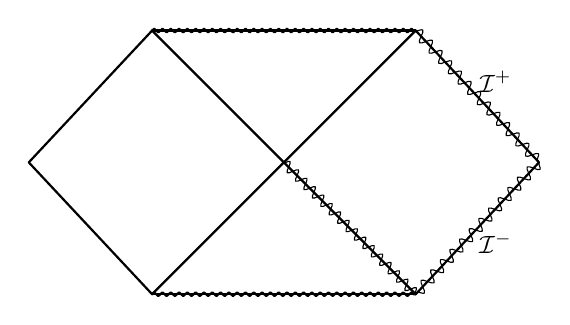
\begin{tikzpicture}[x=1.08cm,y=1.08cm,font=\small,line cap=round,line join=round]
    \coordinate (L) at (-3,0);
    \coordinate (TL) at (-1.55,1.55);
    \coordinate (BL) at (-1.55,-1.55);
    \coordinate (C) at (0,0);
    \coordinate (TR) at (1.55,1.55);
    \coordinate (BR) at (1.55,-1.55);
    \coordinate (R) at (3,0);
    \draw[thick] (L)--(TL)--(C)--(BL)--cycle;
    \draw[thick] (C)--(TR)--(R)--(BR)--cycle;
    \draw[thick,decorate,decoration={zigzag,segment length=3pt,amplitude=.65pt}]
      (TL)--(TR);
    \draw[thick,decorate,decoration={zigzag,segment length=3pt,amplitude=.65pt}]
      (BL)--(BR);
    \draw[thick] (TL)--(TR);
    \draw[thick] (BL)--(BR);
    % Oscillatory wave fronts on null infinity and the white-hole horizon.
    \draw[decorate,decoration={snake,segment length=5.1pt,amplitude=2.0pt}]
      (TR)--(R);
    \draw[decorate,decoration={snake,segment length=5.1pt,amplitude=2.0pt}]
      (R)--(BR);
    \draw[decorate,decoration={snake,segment length=4.3pt,amplitude=1.8pt}]
      (C)--(BR);
    \node[right] at (2.18,.95) {\(\mathcal I^+\)};
    \node[right] at (2.18,-.95) {\(\mathcal I^-\)};
  \end{tikzpicture}
  \caption{A conformal diagram of the extended Schwarzschild spacetime (see
  Figure~12.3) showing the oscillations of a wave of frequency \(\omega\), i.e.,
  \(\mathcal L_\xi\phi=-\ii\omega\phi\). The apparent increase in oscillation
  frequency shown in the figure on \(\mathcal I^+\) at late retarded time (which
  also occurs on \(\mathcal I^+\) at early retarded time and on \(\mathcal I^-\)
  at late and early advanced times) is merely an artifact of the conformal diagram
  caused by the behavior of the conformal factor there. However, the increase in
  frequency shown on the white hole horizon near its crossing point with the black
  hole horizon represents a physical ``infinite blueshift'' singularity of the wave.}
  \label{fig:14.2}
\end{figure}
\endgroup

% Source: Wald GR, physical PDF p. 418
%         (printed p. 405).
% Coverage: Backward propagation through collapsing matter.
% Figures/tables/footnotes: Figure 14.3; no tables or footnotes.
% Status: source-reviewed and compile-clean.
% Uncertainties: none.

\begingroup
\renewcommand{\thefigure}{14.3}
\begin{figure}[htbp]
  \centering
  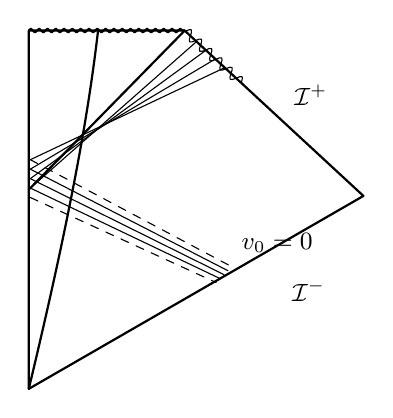
\begin{tikzpicture}[x=1cm,y=1cm,font=\small,line cap=round,line join=round]
    \coordinate (B) at (-1.70,-2.35);
    \coordinate (A) at (-1.70,2.20);
    \coordinate (S) at (.28,2.20);
    \coordinate (R) at (2.55,.10);
    \draw[thick] (B)--(A)--(S)--(R)--cycle;
    \draw[thick,decorate,decoration={zigzag,segment length=3pt,amplitude=.65pt}]
      (A)--(S);
    % Surface of the collapsing body and event horizon.
    \draw[thick] (B) .. controls (-1.10,.15) and (-.92,1.35) .. (-.82,2.20);
    \draw[thick] (-1.70,.18)--(S);
    % Backward-propagated wave fronts.  The upper family arrives from
    % \mathcal I^+; its continuation through the collapsing body accumulates
    % at the point v_0=0 on \mathcal I^-.
    \draw[thin] (-1.68,.20)--(.43,2.06);
    \draw[thin] (-1.68,.32)--(.55,1.95);
    \draw[thin] (-1.68,.44)--(.67,1.84);
    \draw[thin] (-1.68,.56)--(.79,1.73);
    \draw[thin] (-1.68,.20)--(.73,-.95);
    \draw[thin] (-1.68,.32)--(.78,-.90);
    \draw[thin] (-1.68,.44)--(.83,-.85);
    \draw[dashed] (-1.68,.08)--(.68,-1.00);
    \draw[dashed] (-1.68,.56)--(.88,-.80);
    \node[anchor=south west] at (.88,-.74) {\(v_0=0\)};
    \node[right] at (1.55,1.38) {\(\mathcal I^+\)};
    \node[right] at (1.52,-1.10) {\(\mathcal I^-\)};
    \draw[decorate,decoration={snake,segment length=5pt,amplitude=1.8pt}]
      (S)--(1.05,1.49);
  \end{tikzpicture}
  \caption{A conformal diagram of a spherically symmetric spacetime in which
  gravitational collapse to a Schwarzschild black hole occurs, showing the
  oscillations of a wave which behaves as \(e^{-\ii\omega u}\) on
  \(\mathcal I^+\). If one propagates this wave backward into the past starting
  from \(\mathcal I^+\), the part of the wave which propagates through the
  collapsing matter will produce an ``infinite blueshift'' singularity---of the same
  nature as shown on the white hole horizon in Figure~\ref{fig:14.2}---at advanced
  time \(v_0\) on \(\mathcal I^-\).}
  \label{fig:14.3}
\end{figure}
\endgroup


The crucial point is that although we started with the purely positive frequency mode
\(e^{-\ii\omega u}\) at \(\mathcal I^+\), the solution at \(\mathcal I^-\) is
\emph{not} purely positive frequency. Indeed, it is not difficult to show that the
Fourier transform, \(\widetilde\phi\), of \(\phi\) with respect to \(v\) satisfies for
\(\sigma>0\)
\begin{equation}
  \widetilde\phi(-\sigma)
  =-e^{-\pi\omega/\kappa}\widetilde\phi(\sigma)
  \tag{14.3.6}\label{eq:14.3.6}
\end{equation}
(see, e.g., appendix~A of Wald 1975), so the magnitude of the negative frequency
part of \(\phi\) at \(\mathcal I^-\) is the factor \(e^{-\pi\omega/\kappa}\) times the
magnitude of the positive frequency part of \(\phi\). Note that the derivation
of~\eqref{eq:14.3.5} is independent of the details of collapse. Note also that the
decomposition of \(\phi\) into positive and negative frequency parts at
\(\mathcal I^-\) obtained in the case of collapse to a black hole is equivalent to the
decomposition one would obtain in the extended Schwarzschild spacetime using the
affine parameter (rather than the Killing parameter, or any other choice) to define
the notion of positive frequency on the white hole horizon.

To obtain the scattering operators on the one-particle Hilbert space, one should work
with normalized wave packets. Consider a positive frequency wave packet at
\(\mathcal I^+\) composed mainly of frequencies near \(\omega\) and centered on
retarded time \(u\). For large \(u\) (i.e., after the black hole appears to an observer
at infinity to have ``settled down'' to its final static state), the analysis given above
can be applied to this packet and equation~\eqref{eq:14.3.6} will continue to
hold.\footnote{One rather disturbing feature of the analysis should be pointed out.
The mean frequency of the wave packet at \(\mathcal I^-\) increases with advanced
time \(v\) as \(\kappa e^{\kappa v}\) (see Wald 1976), which rapidly becomes very
large, in particular, much larger than the Planck frequency. These ultrahigh
frequencies only enter the intermediate stages of calculation---they do not appear in
any of the final physical predictions---but even so, one may feel uncomfortable that
during the calculation one considers conditions so extreme that the classical wave
propagation used would appear to be very difficult to justify.} It follows directly
from general properties derived in problems~2, 3, and~5 that the expected number of
particles spontaneously created in the state represented by this packet is (Hawking
1975)
\begin{equation}
  \langle N\rangle
  =|t|^2\frac{e^{-2\pi\omega/\kappa}}{1-e^{-2\pi\omega/\kappa}}.
  \tag{14.3.7}\label{eq:14.3.7}
\end{equation}
Here \(|t|^2\) is the square of the Klein--Gordon norm of the part of the wave
packet which would enter the white hole in the extended Schwarzschild solution.
But this is equal to the absorption cross section of the black hole for that mode.
Thus, equation~\eqref{eq:14.3.7} is precisely the formula which would hold for a
perfect blackbody emitter at temperature given by
\begin{equation}
  kT=\frac{\hbar\kappa}{2\pi c}=\frac{\hbar c^3}{8\pi GM},
  \tag{14.3.8}\label{eq:14.3.8}
\end{equation}
i.e.,
\begin{equation}
  T\approx6\times10^{-8}(M_\odot/M)\,\mathrm K,
  \tag{14.3.9}\label{eq:14.3.9}
\end{equation}
% SOURCE ERRATUM: printed ``Boltzman's''; corrected to ``Boltzmann's.''
where \(k\) is Boltzmann's constant and we have restored the \(G\)'s and \(c\)'s.
This similarity of black hole ``emission'' via particle creation with blackbody
emission extends well beyond the agreement~\eqref{eq:14.3.7} in expected numbers
of particles. A complete analysis of the density matrix describing the outgoing state
at infinity shows that it is identical in all aspects to a thermal density matrix at
temperature~\eqref{eq:14.3.8} (Wald 1975; Parker 1975; Hawking 1976).
Furthermore, in the presence of incoming particles the black hole continues to
behave exactly like a blackbody (Panangaden and Wald 1977). The significance of
the fact that black holes behave like perfect blackbodies will be explored further in
the next section.

Note that the temperature of the particles ``emitted'' by the black hole is inversely
proportional to the mass of the black hole. Thus, if energy is added to a black hole,
the temperature decreases, i.e., a black hole has negative specific heat. Negative
specific heats are typical of self-gravitating systems. For example, in Newtonian
gravity, a self-gravitating star composed of an ideal gas has a negative specific heat.

The main modification of the above analysis needed to treat the case of the Kerr
black hole arises from the fact that the Killing field
\(\chi^a=(\partial/\partial t)^a+\Omega_H(\partial/\partial\varphi)^a\),
equation~\eqref{eq:12.3.20}, rather than the stationary Killing field
\((\partial/\partial t)^a\), is normal to the horizon in this case. Consequently, for
an ``initial'' wave at \(\mathcal I^+\) with time dependence \(e^{-\ii\omega u}\)
and angular dependence \(e^{\ii m\varphi}\), the dependence of the solution on
affine parameter along a geodesic which enters the black hole is
\(\exp[\ii(\omega-m\Omega_H)\kappa^{-1}\ln(-\alpha\lambda)]\). For the
non-superradiant modes, the only change in the final expression for the density
matrix is the replacement of \(\omega\) by \(\omega-m\Omega_H\). For the
superradiant modes, the form of the density matrix changes (Wald 1975), but
equation~\eqref{eq:14.3.7} continues to hold with
\(\omega\longrightarrow\omega-m\Omega_H\) provided that \(|t|^2\) is
interpreted to be negative. Because of the frequency shift
\(\omega\longrightarrow\omega-m\Omega_H\) in equation~\eqref{eq:14.3.7}, the
Kerr black hole preferentially loses angular momentum (see Page 1976b for
quantitative details).

It is noteworthy that the thermal nature of black hole emission can be related in a
direct manner to the properties of the Euclidean Schwarzschild solution. As
discussed briefly in section~14.1, in the Euclidean approach to quantum field theory
one seeks to define quantities on a ``Euclidean section'' and then obtain the physical,
spacetime quantities by analytic continuation. In particular, the Feynman propagator
for a field on spacetime is obtained by analytic continuation of the Green's function
on the Euclidean section. (Since the equation for a free field is elliptic rather than
hyperbolic on the Euclidean section, there often will exist a unique Green's function
on the Euclidean section satisfying natural boundary conditions.) In our case, one
is naturally led to examine the properties of the \emph{Euclidean Schwarzschild
solution} obtained by analytically continuing \(t\) to real values of \(\tau=\ii t\) in
equation~\eqref{eq:6.1.44},
\begin{equation}
  \dd s_E^2
  =+\left(1-\frac{2M}{r}\right)\dd\tau^2
   +\left(1-\frac{2M}{r}\right)^{-1}\dd r^2+r^2\dd\Omega^2.
  \tag{14.3.10}\label{eq:14.3.10}
\end{equation}
In Euclidean Schwarzschild space, we again encounter a singularity in the coordinate
components of the metric at \(r=2M\). As we shall see below, this singularity is
again merely a coordinate singularity but its nature is quite different from the
Lorentzian case. To analyze it, we define a new coordinate \(R\) by
\begin{equation}
  R=4M(1-2M/r)^{1/2}.
  \tag{14.3.11}\label{eq:14.3.11}
\end{equation}
Then, we have
\begin{equation}
  \dd s_E^2
  =R^2\dd(\tau/4M)^2+\left(\frac{r}{2M}\right)^4\dd R^2+r^2\dd\Omega^2,
  \tag{14.3.12}\label{eq:14.3.12}
\end{equation}
where now \(r\) is understood to be the function of \(R\) determined by
equation~\eqref{eq:14.3.11}. From equation~\eqref{eq:14.3.12}, it is manifest that
the coordinate singularity at \(R=0\) (i.e., \(r=2M\)) is of the same nature as the
coordinate singularity that occurs at the origin of polar coordinates on the plane,
where now \(R\) plays the role of the radial coordinate and \(\tau/4M\) plays the
role of the angular coordinate. Therefore, a natural choice of manifold structure
for the Euclidean Schwarzschild solution is to periodically identify \(\tau/4M\)---with
period \(2\pi\)---in the region \(r>2M\) and then ``add in'' a single
point\footnote{Since the Schwarzschild manifold is the ``\(R\)-\(\tau\) plane''
crossed with the ``\(\theta\)-\(\varphi\) 2-sphere,'' one, of course, really is
``adding in'' a 2-sphere to the manifold when one adds a point to the
\(R\)-\(\tau\) plane.} in the ``\(R\)-\(\tau\) plane'' to extend the space to
\(R=0\). In this way, one obtains a complete Riemannian manifold
\((M,g_{ab}^E)\) with topology \(M=\mathbb R^2\times S^2\). Note that the
Euclidean Schwarzschild manifold has no region corresponding to the region
\(r<2M\) in the Lorentzian spacetime.

With the above interpretation of the Euclidean Schwarzschild solution, clearly
every continuous function on \(M\) is periodic in \(\tau\) with period \(8\pi M\).
In particular, any Green's function will satisfy this property in each of its variables.
Hence, if the Feynman propagator in the Lorentzian Schwarzschild solution is defined
by analytic continuation of a Euclidean Green's function, it automatically will be
periodic in ``imaginary time'' \(\tau=\ii t\). However, this property of periodicity in
imaginary time is characteristic of a thermal state, as we now shall explain.

Suppose we have an ordinary quantum mechanical system with a time independent
Hamiltonian operator \(H\). The state of thermal equilibrium of the system at
temperature \(kT=\beta^{-1}\) is defined to be that described by the density matrix
\begin{equation}
  \rho=e^{-\beta H}/Z,
  \tag{14.3.13}\label{eq:14.3.13}
\end{equation}
where
\begin{equation}
  Z=\Tr(e^{-\beta H}).
  \tag{14.3.14}\label{eq:14.3.14}
\end{equation}
Furthermore, in the Heisenberg representation, every observable \(O\) evolves with
time by
\begin{equation}
  O(t_0+t)=e^{\ii Ht/\hbar}O(t_0)e^{-\ii Ht/\hbar}.
  \tag{14.3.15}\label{eq:14.3.15}
\end{equation}
In quantum field theory, one in general cannot rigorously define a Hamiltonian
operator \(H\) and, in any case, \(e^{-\beta H}\) would not define a normalizable
density matrix. However, at least in a formal sense, equation~\eqref{eq:14.3.13}
still should describe a state of thermal equilibrium and the field operator
\(\widehat\phi\) should evolve with time via equation~\eqref{eq:14.3.15}. We
define the \emph{thermal Feynman propagator} at temperature \(kT=\beta^{-1}\) by
\begin{equation}
  \ii\Delta_T(x_1,x_2)
  =\Tr\!\left[\rho T(\widehat\phi(x_1)\widehat\phi(x_2))\right]
  =Z^{-1}\Tr\!\left[e^{-\beta H}
    T(\widehat\phi(x_1)\widehat\phi(x_2))\right],
  \tag{14.3.16}\label{eq:14.3.16}
\end{equation}
where, on the right side of this equation, \(T\) denotes the time ordered product
(see equation~\eqref{eq:14.2.22}). Now, suppose that we can analytically continue
\(t\) to imaginary values, \(t=-\ii\tau\), such that equations~\eqref{eq:14.3.15}
and~\eqref{eq:14.3.16} continue to hold. Consider the case where
\(\tau_2-\beta\hbar<\tau_1<\tau_2\) and let \(x_1'\) denote the ``imaginary time
translate'' of \(x_1\) by \(\beta\hbar\), i.e., \(x_1'\) has the same spatial
coordinates as \(x_1\) but has imaginary time coordinate
\(\tau_1+\beta\hbar\). Then, we have
\begin{align}
  \ii\Delta_T(x_1',x_2)
  &=Z^{-1}\Tr\!\left[e^{-\beta H}
      T(\widehat\phi(x_1')\widehat\phi(x_2))\right]\notag\\
  &=Z^{-1}\Tr\!\left[e^{-\beta H}
      \widehat\phi(x_1')\widehat\phi(x_2)\right]\notag\\
  &=Z^{-1}\Tr\!\left[e^{-\beta H}
      \{e^{\beta H}\widehat\phi(x_1)e^{-\beta H}\}
      \widehat\phi(x_2)\right]\notag\\
  &=Z^{-1}\Tr\!\left[\widehat\phi(x_1)e^{-\beta H}
      \widehat\phi(x_2)\right]\notag\\
  &=Z^{-1}\Tr\!\left[e^{-\beta H}\widehat\phi(x_2)
      \widehat\phi(x_1)\right]\notag\\
  &=Z^{-1}\Tr\!\left[e^{-\beta H}
      T(\widehat\phi(x_1)\widehat\phi(x_2))\right]\notag\\
  &=\ii\Delta_T(x_1,x_2).
  \tag{14.3.17}\label{eq:14.3.17}
\end{align}
where the cyclic property of the trace was used in the fifth line. More generally,
when restricted to the strip \(|\tau_1-\tau_2|<\beta\hbar\),
\(\Delta_T(x_1,x_2)\) is periodic in each time variable with period
\(P=\beta\hbar\).

Thus, the Feynman propagator on Schwarzschild spacetime obtained from the
Euclidean Schwarzschild solution is most naturally interpreted as a thermal Feynman
propagator for the field at temperature
\begin{equation}
  kT=\beta^{-1}=\hbar/P=\hbar/8\pi M.
  \tag{14.3.18}\label{eq:14.3.18}
\end{equation}
This suggests the existence of a state of thermal equilibrium of the quantum field at
temperature~\eqref{eq:14.3.18} in Schwarzschild spacetime. This state---or, more
precisely, density matrix---is known as the \emph{Hartle--Hawking vacuum} (Hartle
and Hawking 1976; Israel 1976) and it corresponds to what would result at late times
if a thermal distribution at temperature~\eqref{eq:14.3.18} rather than
\(\lvert0_{\mathrm{in}}\rangle\) was sent in from \(\mathcal I^-\). However,
thermal equilibrium in Schwarzschild spacetime should not be possible unless the
Schwarzschild black hole behaves like a perfect blackbody. Thus, the thermal nature
of particle creation by a Schwarzschild black hole is strongly suggested by the
properties of the Euclidean Schwarzschild solution. Note that this argument for the
thermal properties of a Schwarzschild black hole is applicable to the case of a
nonlinear (i.e., self-interacting) field (Gibbons and Perry 1976; Sewell 1982).

As a result of the thermal particle creation, it is clear that the quantum field carries
energy away from a Schwarzschild black hole. The full stress-energy properties of
the quantum field in Schwarzschild spacetime can be obtained from its stress-energy
operator \(\widehat T_{ab}\). Since the problem of determining \(\widehat T_{ab}\)
and using it to calculate ``back reaction'' effects of the quantum field on the spacetime
is of interest in many applications (particularly, in cosmology), we first shall discuss
these issues in the general context of quantum field theory in curved spacetime, and
then return to the particular case of a black hole.

It is natural to postulate that the stress-energy operator of a quantum field in curved
spacetime is given in terms of the field operator by the same formula as applies
classically, i.e., for the Klein--Gordon quantum field,
\begin{equation}
  \widehat T_{ab}
  =\nabla_a\widehat\phi\nabla_b\widehat\phi
  -\frac12g_{ab}\left[m^2\widehat\phi^2
    +\nabla_c\widehat\phi\nabla^c\widehat\phi\right].
  \tag{14.3.19}\label{eq:14.3.19}
\end{equation}
Unfortunately, this formula requires us to compose two field operators at the same
spacetime point. Since, as mentioned above, \(\widehat\phi\) is well defined only as
a distribution on spacetime, this product is ill defined. Indeed, if one formally
substitutes the mode sum~\eqref{eq:14.2.15} for \(\widehat\phi\) into
equation~\eqref{eq:14.3.19}, the resulting expression one obtains for
\(\widehat T_{ab}\) diverges.

This divergence in the expression for \(\widehat T_{ab}\) also occurs in Minkowski
spacetime. In that case, it is interpreted as arising from the sum of the ``zero-point
energies'' of the infinite number of modes of oscillation of the field. The divergence
is cured by subtracting this zero-point energy from the formal expression for
\(\widehat T_{ab}\) so that the expected stress-energy of the vacuum state vanishes,
\(\langle0\rvert\widehat T_{ab}\lvert0\rangle=0\). This is equivalent to
\emph{normal ordering} the expression for \(\widehat T_{ab}\), i.e., placing all
annihilation operators to the right of creation operators in the formal mode sum
obtained from equation~\eqref{eq:14.3.19}. In this manner, one obtains well defined,
finite expressions for matrix elements of \(\widehat T_{ab}\) between physically
reasonable states.

In curved spacetime, there is, in general, no meaningful notion of an ``instantaneous
vacuum state'' with respect to which one could ``normal order'' the expression for
\(\widehat T_{ab}\). Nevertheless, there exist a number of procedures for
``regularizing'' \(\widehat T_{ab}\), i.e., separating it in a natural way into the sum
of a divergent part and a finite part. Many of these procedures---such as dimensional
regularization (see, e.g., Brown 1977) and zeta-function regularization (Hawking
1977)---are rigorously defined only on a Riemannian manifold (see Wald 1979c), but
at least one of them---namely, ``point-splitting''---also is well defined on Lorentzian
spacetimes (see Fulling 1983 for a summary of results). Unfortunately, the
``divergent part'' of \(\widehat T_{ab}\) cannot be ``absorbed'' into parameters
already present in the theory; i.e., the determination of \(\widehat T_{ab}\) suffers
from the same ``non-renormalizability'' difficulty as is present in full quantum
gravity described in section~14.1 above. Consequently, one finds that one must
introduce two new, nonclassical parameters into the expression for
\(\widehat T_{ab}\) corresponding to the freedom of adding in the identity operator
times multiples of the two conserved local curvature terms\footnote{These terms are
the ones obtained by variation of the actions \(\int R^2\) and
\(\int R_{ab}R^{ab}\) with respect to the metric (see appendix~E). Most
regularization prescriptions yield a precise value for one combination of these
parameters, but since different prescriptions sometimes lead to different values, it
probably is wisest to regard both of them as undetermined.} of dimension
\((\text{length})^{-4}\). Thus, there is a two-parameter ambiguity in the expression
for \(\widehat T_{ab}\). However, \(\widehat T_{ab}\) satisfies a list of physically
reasonable properties which uniquely determine it up to this two-parameter
ambiguity (Wald 1977b, 1978b), so it appears that this is the only ambiguity present.

An important feature of the expectation value
\(\langle\Psi\rvert\widehat T_{ab}\lvert\Psi\rangle\) of the quantum
stress-energy operator \(\widehat T_{ab}\) in a state \(\Psi\) is that it need not
satisfy any of the energy conditions that may be satisfied by the classical
stress-energy tensor. Indeed, even in flat spacetime one can find states where the
expectation value of the normal ordered Klein--Gordon stress-energy operator has
negative energy density in a region of spacetime, even though the energy density of
the classical stress-energy tensor of a Klein--Gordon field is manifestly positive
definite everywhere for all field configurations (see problem~6). Thus, properties
which hold in classical general relativity by virtue of energy conditions satisfied by
matter will not necessarily hold for quantum fields. This has important consequences
for the black hole area theorem, as will be discussed further in the next section.

In the context of quantum field theory in curved spacetime, it is natural to postulate
that the back-reaction effects of the quantum field on the gravitational field will be
governed by the semiclassical Einstein equation,
\begin{equation}
  G_{ab}=8\pi\langle\Psi\rvert\widehat T_{ab}\lvert\Psi\rangle,
  \tag{14.3.20}\label{eq:14.3.20}
\end{equation}
i.e., it is physically possible for the spacetime to be \((M,g_{ab})\) and for the
quantum field to be in state \(\Psi\) on \((M,g_{ab})\) if and only if
equation~\eqref{eq:14.3.20} is satisfied. Actually, equation~\eqref{eq:14.3.20}
would \emph{not} be expected to arise as the lowest approximation to a quantum
field theory of gravity coupled to a matter field. This is because in the full theory
one would expect to have
\(\langle\widehat G_{ab}\rangle=8\pi\langle\widehat T_{ab}\rangle\) hold
exactly, where \(\widehat G_{ab}\) is the Einstein operator and the state implicit in
the expectation values now includes the degrees of freedom of the gravitational
field. Furthermore, one would expect that \(\widehat G_{ab}\) would be given in
terms of the metric operator by the same formula as holds classically,
\(\widehat G_{ab}=G_{ab}[\widehat g_{cd}]\). However, since \(G_{ab}\) is a
nonlinear function of \(g_{cd}\) we expect
\(\langle\widehat G_{ab}\rangle\ne
G_{ab}[\langle\widehat g_{cd}\rangle]\). Indeed, if we write
\(\widehat g_{ab}=g_{ab}^{c}\widehat I+\widehat h_{ab}\)---where
\(g_{ab}^{c}\) is a classical solution of Einstein's equation and \(\widehat I\) is
the identity operator---and if we keep only terms quadratic in \(\widehat h_{ab}\)
in the formula for \(\widehat G_{ab}\), then \(\langle\widehat G_{ab}\rangle\)
and \(G_{ab}[\langle\widehat g_{ab}\rangle]\) will differ by
\(-8\pi\langle\widehat t_{ab}\rangle\), where \(\widehat t_{ab}\) is given in
terms of \(\widehat h_{ab}\) by a formula very similar to that for
\(\widehat T_{ab}\) in terms of \(\widehat\phi\). (See
equations~\eqref{eq:4.4.54} and~\eqref{eq:4.4.51} for an explicit formula for
\(t_{ab}\) in the case \(g_{ab}^{c}=\eta_{ab}\).) Consequently, in the lowest
approximation to a full quantum field theory of gravity coupled to matter, one would
expect to get the additional term \(8\pi\langle\widehat t_{ab}\rangle\) appearing
on the right-hand side of equation~\eqref{eq:14.3.20}, and the contribution from this
term should be comparable to that of \(\langle\widehat T_{ab}\rangle\). One can
interpret this fact as saying that the quantum back-reaction effects caused by
\emph{gravitons} (i.e., the quantized degrees of freedom of the linearized
gravitational field) are as important as that of any other quantum field, and thus
should not be neglected in equation~\eqref{eq:14.3.20}. Nevertheless, one can
justify equation~\eqref{eq:14.3.20} in terms of a systematic approximation to a full
quantum field theory including gravitation as follows. If we have \(N\) matter fields
present, then, roughly speaking, the effects of the matter fields will be \(N\) times as
important as that of the gravitons. Hence, in the limit of large \(N\), the neglect of
the gravitons should be justified, and one will obtain equation~\eqref{eq:14.3.20}
(with a coefficient of \(N\) on the right-hand side) as the lowest approximation in a
``\(1/N\) expansion'' of the full theory of quantum gravity coupled to matter. In any
case, equation~\eqref{eq:14.3.20} should at least provide a qualitative indication of
the back-reaction effects produced by quantum fields on the gravitational field.

Unfortunately, the dynamics predicted by equation~\eqref{eq:14.3.20} is drastically
different from classical general relativity. There exist many unphysical solutions of
equation~\eqref{eq:14.3.20} in which the spacetime curvature is initially small but
exponentially grows with time with time scale of order of the Planck time. Indeed,
Horowitz (1980) has shown that for any massless quantum field,
equation~\eqref{eq:14.3.20} predicts this type of instability of Minkowski spacetime.
Thus, the situation is very similar to that which occurs in the classical
electrodynamics of a point charge when radiation reaction is taken into account (see,
e.g., Jackson 1962). There, the ``small'' correction to the equations of motion caused
by radiation reaction leads to new ``runaway'' solutions. In the case of
electrodynamics, one still can make physically sensible predictions by simply
disregarding these runaway solutions, although doing so requires putting constraints
on the initial conditions of the point charge which depend upon what external forces
are to be applied in the future. It appears that it will be much more difficult to
develop procedures for extracting the physically sensible solutions of
equation~\eqref{eq:14.3.20}.

In the case of a Schwarzschild black hole (or, more generally, in any vacuum
spacetime, \(R_{ab}=0\)) the two local curvature terms which enter the formula for
\(\widehat T_{ab}\) with undetermined coefficients vanish identically. Hence
\(\widehat T_{ab}\) is completely well defined in the Schwarzschild spacetime. The
value of \(\langle\widehat T_{ab}\rangle\) in the ``Hartle--Hawking vacuum'' has
been calculated analytically on the horizon by Candelas (1980) and computed
numerically near the black hole by Fawcett (1983). The magnitude of the Kruskal
coordinate components of \(\langle\widehat T_{ab}\rangle\) near the black hole are
found to be of order \(1/M^4\) in Planck units \(G=c=\hbar=1\), as expected on
dimensional grounds. Since the background curvature is of order \(1/M^2\), for
\(M\gg1\) (i.e., in cgs units, \(M\gg10^{-5}\,\mathrm g\)), the quantum field
should make only a small correction to the structure of the black hole. The energy
flux into the black hole is found to be negative, as must be the case since the
``Hartle--Hawking vacuum'' is time independent and the energy flux at future null
infinity is positive. Such a negative energy flux is possible since, as mentioned
above, \(\langle\widehat T_{ab}\rangle\) need not satisfy any of the classical energy
conditions.

As discussed above, serious difficulties arise when one tries to use
equation~\eqref{eq:14.3.20} to calculate the back-reaction effects. However, on
physical grounds, one expects that the main back-reaction effect of the quantum field
will be to cause the black hole to lose mass at the same rate at which energy is
radiated to infinity by particle creation. This can be calculated by multiplying
\(\langle N\rangle\), equation~\eqref{eq:14.3.7}, by \(\omega\) and summing over
modes. Since the emission is of a blackbody nature, if the absorption cross section
\(|t|^2\) for each mode were the same as for a black sphere of radius \(R\) in
Minkowski spacetime and if \(kT\gg\hbar cR^{-1}\), the energy flux for a massless
field with two degrees of freedom would be given by Stefan's law,
\(\dd E/\dd t=\sigma T^4A=\sigma T^4 4\pi R^2\), where
\(\sigma=\pi^2k^4/60\hbar^3c^2\) is the Stefan--Boltzmann constant. In the
geometric optics approximation, the black hole does absorb just like a black sphere
of radius \(R=3^{3/2}M\) (see chapter~6). However, since the relevant modes in
black hole particle creation have frequencies of order \(M^{-1}\) (i.e., one has
\(kT\sim\hbar cR^{-1}\)) one must use physical optics\footnote{The failure of
geometrical optics to accurately describe wave propagation well outside the horizon
(where most of the scattering occurs) should be distinguished from the validity of
geometrical optics to describe wave propagation very near the horizon, as used
above in the calculation of particle creation.} (i.e., exact wave propagation) to
compute \(|t|^2\) accurately. Nevertheless, Stefan's law provides a correct order of
magnitude estimate for the energy flux from a black hole. Hence, ignoring numerical
factors, we find that in Planck units, the mass loss rate of the black hole is
approximately
\begin{equation}
  \frac{\dd M}{\dd u}\sim-AT^4\sim-M^2(1/M)^4=-\frac1{M^2}.
  \tag{14.3.21}\label{eq:14.3.21}
\end{equation}
Thus, as the black hole loses mass, the increase in temperature more than
compensates for the decrease in area, and the energy loss due to particle creation
occurs at a faster rate. Integrating equation~\eqref{eq:14.3.21}, we obtain the
striking conclusion that a black hole should radiate all of its mass in a finite time
\(\tau\) given in Planck units by
\begin{equation}
  \tau\sim M^3.
  \tag{14.3.22}\label{eq:14.3.22}
\end{equation}
In cgs units, \(M^3\) is \(\sim10^{71}(M/M_\odot)^3\,\mathrm s\), so the lifetime
for total ``evaporation'' of a black hole of a solar mass or larger is enormously
greater than the age of the universe.

% Source: Wald GR, physical PDF p. 426
%         (printed p. 413).
% Coverage: Collapse followed by complete black-hole evaporation.
% Figures/tables/footnotes: Figure 14.4; no tables or footnotes.
% Status: source-reviewed and compile-clean.
% Uncertainties: none.

\begingroup
\renewcommand{\thefigure}{14.4}
\begin{figure}[htbp]
  \centering
  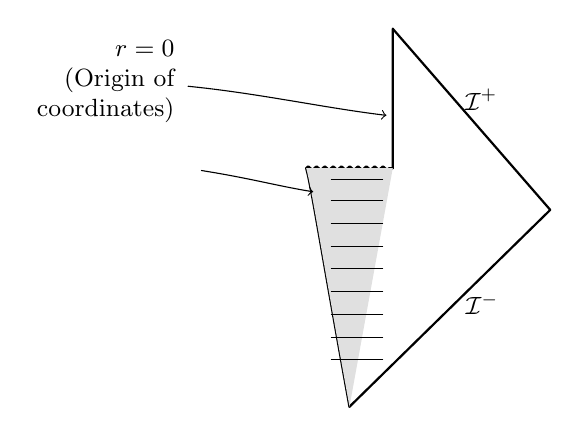
\begin{tikzpicture}[x=1cm,y=1cm,font=\small,line cap=round,line join=round]
    \coordinate (B) at (0,-2.35);
    \coordinate (R) at (2.55,.15);
    \coordinate (T) at (.55,2.45);
    \coordinate (S) at (.55,.68);
    \coordinate (C) at (-.55,.68);
    \draw[thick] (B)--(R)--(T)--(S);
    \draw[thick] (S)--(T);
    \draw[thick,decorate,decoration={zigzag,segment length=3pt,amplitude=.65pt}]
      (C)--(S);
    % Surface of the collapsing matter and shaded black-hole region.
    \draw[thick] (B) .. controls (-.38,-.25) and (-.48,.42) .. (C);
    \path[fill=black!12] (B) .. controls (-.38,-.25) and (-.48,.42) .. (C)
      -- (S) -- cycle;
    \foreach \yy in {-1.75,-1.47,-1.18,-.89,-.60,-.31,-.02,.27,.54}
      \draw[thin] (-.23,\yy)--(.42,\yy);
    \draw[->] (-2.05,1.72) .. controls (-1.15,1.63) and (-.35,1.45) .. (.47,1.35);
    \draw[->] (-1.88,.65) .. controls (-1.25,.55) and (-.90,.45) .. (-.46,.38);
    \node[left,align=right] at (-2.10,1.78) {\(r=0\)\\(Origin of\\coordinates)};
    \node[right] at (1.34,1.55) {\(\mathcal I^+\)};
    \node[right] at (1.35,-1.05) {\(\mathcal I^-\)};
  \end{tikzpicture}
  \caption{A conformal diagram of a spacetime in which a black hole is produced
  by the collapse of matter and ``evaporates'' as a result of the particle creation
  process.}
  \label{fig:14.4}
\end{figure}
\endgroup


However, if any primordial black holes of mass \(\sim5\times10^{14}\,\mathrm g\)
were produced in the early universe, they would be undergoing the final stages of
evaporation now (Page 1976a), and any primordial black holes of smaller mass would
have already evaporated. Since the temperature of a black hole becomes large as
evaporation occurs, a significant amount of \(\gamma\)-radiation would result if many
black holes of mass \(\lesssim5\times10^{14}\,\mathrm g\) were produced in the
early universe. As already mentioned at the end of section~12.1, no such contribution
to the \(\gamma\)-ray background has been observed (Page and Hawking 1976), so it
appears that we do not have a sufficient number of low mass primordial black holes
in our universe to be able to observe the effects of black hole evaporation.

By the time the black hole has evaporated down to the Planck mass, we cannot
expect the approximation of treating gravity classically to be valid, and a description
% SOURCE ERRATUM: printed ``await to complete theory''; corrected to
% ``await a complete theory.''
of what occurs at that stage will have to await a complete theory of quantum gravity.
However, it seems natural to expect that the black hole will totally disappear at the
end of the process, rather than, say, leaving behind a Planck-size black hole remnant.
The causal structure of a spacetime in which a black hole is formed and then
evaporates completely is illustrated in Figure~\ref{fig:14.4}.

Assuming that total evaporation occurs, we mention two important consequences.
First, it appears that conservation of baryons (and/or leptons) can be grossly violated
in the process of collapse to a black hole followed by evaporation even if baryon
number (and/or lepton number) is conserved locally; namely, we can form the black
hole out of matter with a large net baryon number (e.g., purely out of neutrons, with
no antineutrons). The black hole uniqueness theorems discussed at the end of
section~12.3 strictly apply only to the case where certain classically describable
fields are present, but they strongly suggest that the black hole produced by the
collapse of baryons will be indistinguishable from one produced by the collapse of
antibaryons. Hence, in the particle creation process, there should be no preferential
production of baryons over antibaryons and, indeed, in any case most of the mass of
the black hole should be radiated away by massless particles carrying no baryon
number. Thus, at the end of the evaporation process, the net baryon number should
be very nearly zero and a large change in baryon number will have occurred.

Second, as discussed above, the particles reaching infinity during the evaporation
process are described by a density matrix. The use of a density matrix here is purely
for convenience, since the joint state of the particles entering the black hole together
with those reaching infinity is pure, provided, of course, that the incoming state is
pure. However, if the black hole evaporates completely as in Figure~\ref{fig:14.4},
then the \emph{total} state of the system should be described by a density matrix.
Roughly speaking, the correlations with the particles reaching infinity should
propagate into the black hole singularity and be lost forever when the black hole
disappears. Thus, it appears that in the process of black hole formation and
evaporation, an initial pure state can evolve to a final density matrix (Hawking 1976;
Wald 1980; see Page 1980 for a differing view). This shows that a form of time
reversal asymmetry must be present, since an initial density matrix never can evolve
to a final pure state, although a physically meaningful form of time reversal symmetry
may still hold (Wald 1980). The existence of time reversal asymmetry in the laws of
quantum gravity has been suggested on other grounds by Penrose (1979).
Furthermore, the evolution of a pure state to a density matrix in the process of black
hole formation and evaporation may be closely related to issues in quantum
measurement theory (Penrose 1981).

Finally, we briefly describe a further result which shows a connection between
particle creation near a black hole and properties of the ordinary vacuum state of a
quantum field in Minkowski spacetime. This result also gives insight into the physical
meaning of ``particles'' in curved spacetime and the reasons for the mathematical
ambiguities in their definition.

The close mathematical analogy between the ``Rindler wedge'' of Minkowski
spacetime and the region \(r>2M\) of Schwarzschild spacetime already has been
displayed at the end of chapter~6. Indeed, there we used the extension of Rindler
spacetime to Minkowski spacetime to motivate the Kruskal extension of
Schwarzschild spacetime. One can define a quantum field theory in Rindler spacetime
by using the Rindler time coordinate, \(t_R\), rather than a Minkowski time
translation coordinate, \(t_M\), to define the notion of ``positive frequency.'' In
other words, we may ``quantize'' the field in (a wedge of) Minkowski spacetime by
using a ``boost'' rather than an ordinary time translation as our timelike Killing
vector field. These two notions of ``positive frequency'' differ, so one is led to
distinct notions of ``Rindler particles'' and ``Minkowski particles'' (Fulling 1973).
The relation between the characterization of states of the quantum field in terms of
Rindler particles as compared with their characterization in terms of Minkowski
particles can be found by obtaining the Bogoliubov transformation between Rindler
and Minkowski annihilation and creation operators, using the same procedure as in
the case of true particle creation described in the previous section. Since the relation
between Rindler time and Minkowski time is essentially the same as that holding near
the horizon between Schwarzschild time and Kruskal time, it should not be surprising
that the Minkowski positive and negative frequency parts of a solution which
oscillates in Rindler time like \(e^{-\ii\omega t_R}\) are, again, related by
equation~\eqref{eq:14.3.6}. In close mathematical analogy with the calculation of
true particle creation in the Schwarzschild spacetime, it is found here that the
ordinary Minkowski vacuum \(\lvert0\rangle\) is formally represented by a thermal
density matrix of Rindler particles.

A physical interpretation of this result was provided by Unruh (1976). He showed
that a particle detector which uniformly accelerates---i.e., travels along a trajectory
of a boost Killing field---is sensitive to the Rindler particles associated with that
Killing field. This is most easily seen by considering a simple model of a particle
detector consisting of an ordinary nonrelativistic quantum mechanical system (e.g.,
a particle in a box) linearly coupled to the quantum field. Detection of a particle is
said to occur if a transition to a higher energy state occurs in the quantum mechanical
system. From ordinary time-dependent perturbation theory, when the quantum field
is in the ordinary Minkowski vacuum state, \(\lvert0\rangle\), the rate (i.e.,
probability per unit time) for a transition upward in energy by \(E\) for an
accelerating point detector is found to be (see Unruh 1976 or DeWitt 1979)
\begin{equation}
  R(E)\propto\lim_{T\to\infty}\frac1T
  \int_{-T}^{T}\!\int_{-T}^{T}
  e^{-\ii E(t_R-t_R')}
  \langle0\rvert\widehat\phi[x(t_R)]\widehat\phi[x(t_R')]\lvert0\rangle
  \,\dd t_R\,\dd t_R',
  \tag{14.3.23}\label{eq:14.3.23}
\end{equation}
where \(t_R\) has been scaled so that it agrees with proper time along the world
line, \(x(t_R)\), of the accelerating particle detector. Thus, the transition probability
is directly related to a Fourier transform of the vacuum expectation value of the
product of field operators, where this Fourier transform picks out a positive
frequency component with respect to \(t_R'\) and a negative frequency component
with respect to \(t_R\). However, for an accelerating detector these ``positive and
negative frequency parts'' are measured with respect to Rindler time rather than
Minkowski time. Although by equation~\eqref{eq:14.2.13},
\(\widehat\phi\lvert0\rangle\) has no positive frequency part with respect to
Minkowski time and \(\langle0\rvert\widehat\phi\) has no negative frequency part
(which accounts for why an inertial particle detector does not detect particles), they
\emph{do} have such positive and negative frequency parts with respect to Rindler
time. This corresponds precisely to the above representation of the Minkowski
vacuum as a thermal state of Rindler particles. Thus, Unruh (1976) found that an
accelerating particle detector in Minkowski spacetime would behave as though it
were placed in a thermal bath of ``real'' particles, with temperature given by
\begin{equation}
  kT=\frac{\hbar a}{2\pi c}.
  \tag{14.3.24}\label{eq:14.3.24}
\end{equation}
Thus, the ordinary vacuum state in Minkowski spacetime is seen by an accelerating
observer to possess thermal properties which are formally very similar to the thermal
effects resulting from true particle creation by a black hole. Unfortunately, in cgs
units, equation~\eqref{eq:14.3.24} reads
\begin{equation}
  T\approx4\times10^{-23}a\,\mathrm K,
  \tag{14.3.25}\label{eq:14.3.25}
\end{equation}
so it is clear that this effect is much too small to be perceived by an ordinary
laboratory detector. However, the effect of this thermal bath on the spin of
accelerating electrons may be measurable (Bell and Leinaas 1983). Further
discussion of this effect from the viewpoint of an inertial observer is given by Unruh
and Wald (1984).

Thus, the ``Rindler particles'' defined by using a nonstandard notion of positive
frequency in Minkowski spacetime are seen to be associated with true physical
effects. Rindler particles are ``real'' to accelerating observers! This shows that
different notions of ``particle'' are useful for different purposes. Therefore, in a
general curved spacetime where no timelike Killing field is present, it should not be
surprising that there is no natural, universally applicable procedure for defining
particles and that, in a given spacetime, different constructions (such as constructions
using affine parameter or Killing parameter on the horizon of a black hole) will define
different notions of particles. Although the notion of particles is very convenient for
many purposes, it is not an essential ingredient of quantum theory. Physical
predictions always can be expressed in terms of matrix elements
\(\langle\Phi\rvert O\lvert\Psi\rangle\) of an operator \(O\) between states
\(\Phi\) and \(\Psi\), such as in equation~\eqref{eq:14.3.23} or
equation~\eqref{eq:14.3.20}. These predictions will not depend upon how \(\Phi\)
and \(\Psi\) are labeled in terms of particle states.

A similar analysis of the behavior of a particle detector in Schwarzschild spacetime
shows that when the field is in the Hartle--Hawking vacuum state, a stationary
detector at any radius \(r>2M\) will behave as though immersed in a thermal bath at
temperature
\begin{equation}
  kT=\frac{\hbar\kappa}{2\pi cV},
  \tag{14.3.26}\label{eq:14.3.26}
\end{equation}
where \(V=(-\xi^a\xi_a)^{1/2}\) is the redshift factor appropriate to that radius.
Far from the black hole (\(r\longrightarrow\infty\)) we have
\(V\longrightarrow1\), and the effect may be interpreted as the response of the
detector to the ``real'' particles produced by the black hole (as well as those
incoming from \(\mathcal I^-\)). Near the black hole
(\(r\longrightarrow2M\)) we have \(\kappa/V\longrightarrow a\), where \(a\) is
the proper acceleration of the detector (see equation~\eqref{eq:12.5.18}), and the
effect (which becomes divergent at the horizon) may be interpreted as being due to
the acceleration of the detector. A freely falling detector sees essentially no
particles near the black hole (Unruh 1977), in accordance with the negligible
stress-energy \(\langle\widehat T_{ab}\rangle\) of the quantum field near the
horizon.
